\section{\sysname}
\label{sec:system}
% Basic what it is
\sysname is a slim, batteryless, occupancy monitoring enabling sensor platform mounted to the top of a doorframe that is powered by energy harvested from two arrays of indoor solar panels pointed at the floor.
The panels serve two roles: 1)~energy harvester and 2)~sensor.
These panels gather the \textbf{energy} needed for computation, sensing, and signaling while also providing the \textbf{signal} that \sysname uses to detect when a person walks through the doorway.
\sysname records the time and direction---entry or exit---of each doorway event and stores this information in non-volatile memory for later processing.


\noindpar{Design Goals:} Intermittent power supplies coupled with confounding factors of human based sensing combine to make designing an intermittently powered occupancy sensor challenging.
We designed \sysname to meet the following design goals which address specific challenges:
\begin{enumerate}
	\item \textbf{Availability:} Doorway events can occur at any time.
	While many intermittent sensors are able to gather data opportunistically as energy is available, \sysname is designed to conserve its harvested energy, so that it is available to detect ephemeral doorway events, whenever they occur.
	\item \textbf{Variable lighting conditions:} Indoor lighting conditions change throughout the day, due to human behavior and the movement of the sun.
	We have designed \sysname to work in a range of different lighting conditions by using detection circuits that respond to change in light level, independent of the absolute amount of light, as well as tuning mechanisms built into the prototype.
	\item \textbf{Variable human characteristics:} An effective occupancy sensor should work well in spite of variations in clothing, hair, height, walking speed, and skin color. By focusing on changes in total reflected light, \sysname can be robust to these human variations.
	\item \textbf{Form factor:} We want \sysname to be easy to deploy, to fit unobtrusively inside any door frame, and avoid contact with doors (on frames with doors). We could harvest more energy by wrapping \sysname around the doorframe, but the system would be more expensive, harder to deploy, and more likely to interfere with doors, while changing the aesthetics of the doorway.
\end{enumerate}

\noindpar{What \sysname is not.}
We also want to be clear about what \sysname is \emph{not}.
\sysname is \emph{not} a security device.
\sysname helps building owners and managers understand how people move through buildings, but it is \emph{not} designed to thwart malicious behavior.
We can easily trick \sysname with a flashlight or reflective materials, and we can disable it completely by covering its solar panels or turning off the lights.
Users looking to prevent shenanigans or tomfoolery should use a different device.
Users looking for a long-lived, low-maintenance, best-effort batteryless occupancy sensor for monitoring normal behaviors should read on.

% fig refs
An overview of the \sysname architecture is shown in \figref{fig:overview} and our \sysname prototype device is shown in \figref{fig:prototype}.
% Intro the rest of the section
We detail our approach to meeting these design goals and answering their associated challenges in the rest of the section~--- specifically we describe the \sysname architecture and design, the detection mechanism, and the energy management operations.


\begin{figure}[t]
\centering
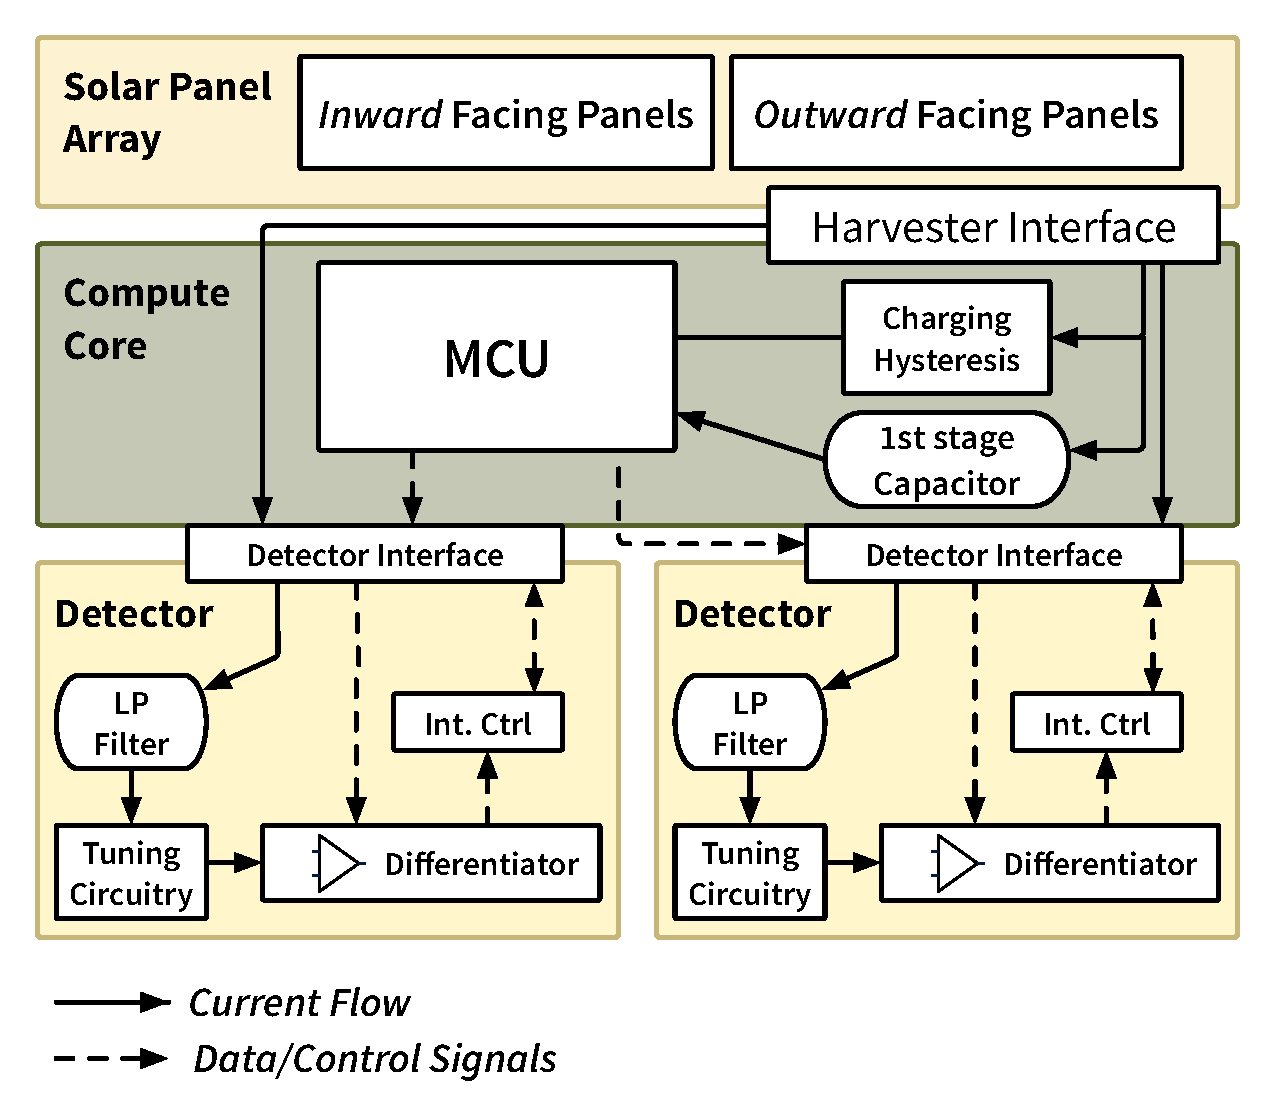
\includegraphics[width=\columnwidth]{figs/overview.pdf}
\caption{The \sysname architecture overview. \sysname uses the energy and signal from two sets of solar panels to both power the sensor and detect people passing into and out of a doorway. Two detector circuits each monitor half of the solar panels mounted in series that face inward, and outward in the doorway. On detection, the detectors wake up the MCU to process, log, or communicate occupancy information.  \label{fig:overview}}
\end{figure}


\subsection{Energy Harvesting and Management}
\sysname takes advantage of the ubiquity of indoor light in homes and offices.
Solar panels are spread across the top of the door frame in a custom 3D printed case, pointing down at the floor.
Pointing the panels downward is not ideal for energy harvesting, but it is ideal for detecting doorway events and provides a slim, easy-to-deploy form factor.

\sysname uses federated energy storage~\cite{jhester:ufop:sensys}. \fxnote{Is this sentence complete? My brain wants more here such as "uses federated energy storage to...", but its probably ok as is. no telling at this hour.  Maybe better to join it somehow with the second sentence.. -NT]}
Energy harvested from all of the solar panels is fed into a common first-stage storage capacitor and then automatically federated to its peripherals.
\sysname currently supports slots for two peripherals, a Texas Instruments CC1101 radio and an ultrasonic rangefinder.  We plan to add additional sensors to our design in the near future. These sensors are not used in the evaluation of our prototype.
Federating energy allows us to prioritize detection and computation while saving up energy for more energy-expensive radio transmissions.
It also improves harvesting efficiency and allows separation of peripherals without fear of the microcontroller losing power.


\subsection{Detection}
\label{sec:detection}

\begin{figure*}[t]
	\centering
	\begin{subfigure}[b]{0.5\textwidth}
		\centering
		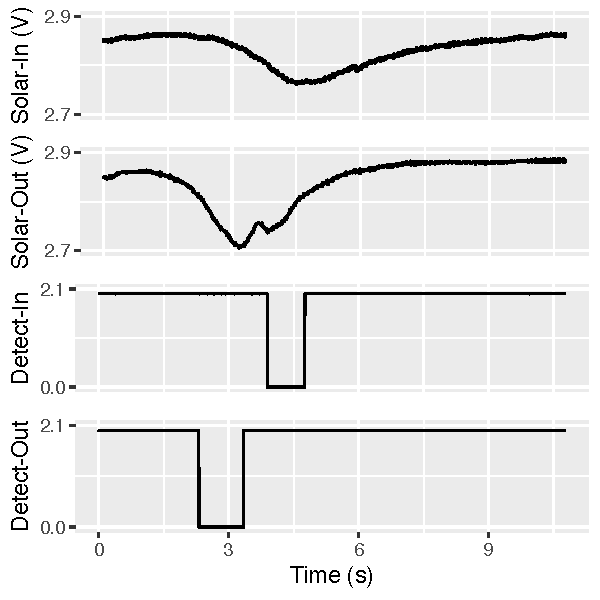
\includegraphics[width=\columnwidth]{figs/tracesin.pdf}
		\caption{Walking in.}
		\label{fig:tracesin}
	\end{subfigure}%
	%
	\begin{subfigure}[b]{0.5\textwidth}
		\centering
		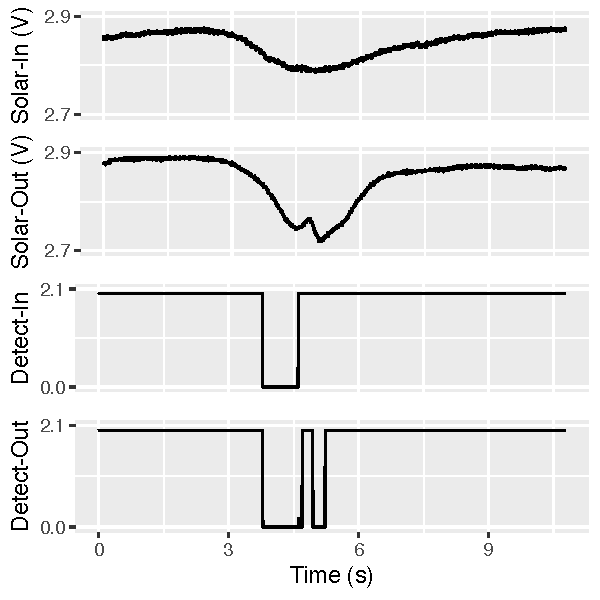
\includegraphics[width=\columnwidth]{figs/tracesout.pdf}
		\caption{Walking out.}
		\label{fig:tracesout}
	\end{subfigure}
	\caption{ These traces show example solar panel voltages and detector outputs over time when a person walks through a \sysname-enabled doorway. The top traces show how the solar panel's voltages are deformed during the doorway event. The detector triggers are used to wake up the microcontroller and detect events and their direction. The angling of the panels cause the inward facing and outward facing detectors to trigger at different times depending on the direction the person is walking.\label{fig:traces}}
\end{figure*}

%\fxnote{[It would be nice to do this data driven off some traces gathered. Simulate, essentially, just by doing some light math. So how do we capture the waveforms when we trigger the wakeup? - JDH]}

%what happens when a person walks through.
When someone walks under \sysname, he or she blocks some of the reflected light hitting the solar panels.
In \figref{fig:traces}, the ``solar'' trace on top shows how the voltage from the solar panels changes during a doorway event.
Doorway events have a characteristic ``W'' shape because the person passing through the doorway first breaks the light reflected from the origin room and then breaks the light coming from the destination room.
The voltage increases when the person is directly under \sysname, and light from both sides is momentarily able to reach the panels.


In order to detect a doorway event, we could use an ADC to continuously measure the solar panel voltage over time and analyze those readings to detect the appropriate ``W'' shape.
Voltage levels and waveform shapes vary with lighting conditions, especially when one side of the doorway has more natural light, and this approach would require sophisticated signal analysis and prohibitive energy consumption.

Instead, \sysname uses a \textbf{detection circuit} that wakes up the microcontroller when it detects a significant change in the solar panel voltage over a short period of time.
This circuit consists of a passive differentiator circuit\footnote{A passive differentiator is essentially a first-order capacitive high-pass filter with the cut-off frequency set well above the highest frequencies in the signal.} with its output fed into a comparator.
This combination produces a square wave with transitions that occur when the solar voltage either increases or decreases faster than a set rate.
\figref{fig:traces} shows example traces from both a high-to-low detection circuit (detects rapid decrease) and a low-to-high detection circuit (detects rapid increase).
In practice we use high-to-low detection circuits exclusively to detect the beginning of a doorway event.

\begin{figure}[t]
\centering
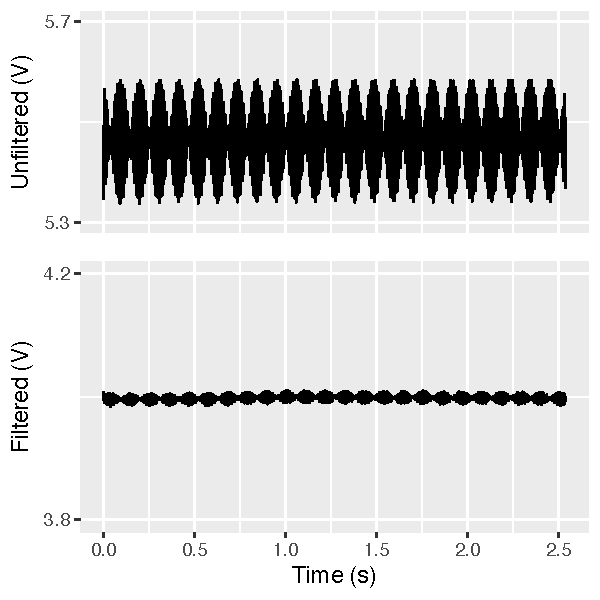
\includegraphics[width=\columnwidth]{figs/flicker.pdf}
\caption{These plots show the impact of the solar signal to \sysname both before and after it the system filters the signal by passing it through the differentiator and the harvestor.  \label{fig:flicker}}
\end{figure}


\noindpar{Removing light flicker.}
Many fluorescent indoor lights flicker at either \SI{60}{\hertz} or higher.
These fluctuations are a much higher frequency than those we want to detect, and they can confuse the detection circuit and produce many false positives unless they are filtered out.
We add a low-pass filter to remove noise above \SI{10}{\hertz} from the solar panel signal.  \figref{fig:flicker} shows the impact of the noise to the light signal both before and after filtering out the higher frequencies from the signal.

\noindpar{Isolating harvesting from sensing.}
If connected directly, \sysname's harvesting and event detection circuits conflict in two important ways.
First, the harvesting circuit stores harvested energy in a \SI{100}{\micro\farad} capacitor---a size that ensures that \sysname can store enough energy for short-term tasks and dampens the low-frequency voltage fluctuations that we need in order to detect doorway events.
Second, short-term power spikes from interrupt service routines and other computation cause high-frequency dips in the solar voltage, which can confuse the detection circuits.
We address both of these challenges by adding an additional low-pass filter between the detection and harvesting circuits, which isolates the solar panel from the load, and allows the solar panel voltage (after the initial flicker filter) to fluctuate over a wider range in response to doorway events with less interference from the storage capacitor, the microcontroller power draw, and the differentiatior circuit power draw.

\noindpar{Detecting movement direction.}
In order to detect the direction that the person is moving, \sysname's solar panels are divided into two groups---one group angled slightly inward and the other group angled outward.
Every other panel is angled facing outward, with the other facing inward.
Each group of panels has its own detection circuit (differentiator, comparator, and low pass filter) and can wake up the microcontroller independent of the other group.

Ideally, when a person walks into a room, the panels tilted outward will react before the inward facing panels and vice versa.
In practice, this is not always the case, due to uneven lighting that can make one detector circuit more sensitive than its counterpart; however, tilting the panels does consistently effect the timing of the interrupts, which we use to determine in what direction the person was moving.

\noindpar{Detection algorithm:}
During normal operation, when \sysname is not in a doorway event, the MCU remains in deep sleep (or if there is not enough energy stored, is in brown-out).
While in deep sleep, the MCU is only triggered awake by the differentiator circuits going from low to high---designating the beginning of a doorway event, from the change in solar harvesting energy from the light occluded by a person walking through the doorway.
Once triggered, the MCU starts a timer (a few seconds), and records the time at which the interrupt occurred, then goes into sleep mode, waking up throughout the doorway event to capture the length of time between each differentiators status change (from LOW to HIGH and vice-versa).
Multiple interrupts often fire during a single doorway event, and the timer defines the boundaries for what will be considered part of the event.

Times are recorded for the first falling edge interrupt and last recorded rising edge for both solar panel groups.
When the timer fires, both solar panel groups' end times are compared to determine the direction of the event and start and end times are compared to determine the duration of the event, and then determine whether the doorway event was an entry or exit.


In rare cases, only one detector will detect the change.
These events are reported as partial events, which don't have a direction.
Partial doorway events can occur when a person walks by the doorway but not through it (close enough to interfere with one panel group).


%\subsection{Communication and Infrastructure}
%\fxnote{[Remove this - JDH]}

%\subsection{Adaptation}
%\fxnote{[Remove this - JDH]}

%\sysname dynamically changes task sets depending on energy availability - attempting to assign higher energy tasks when energy is more available in the environment and assigning lower energy tasks assigned when energy is scarce in the environment. \fxnote{[Does not do this, need to remove - JDH]}
%These tasks correspond to different tiers of quality of service (QoS) of the application, with the highest level providing real time event marking on door traffic coupled with person identification using heights, hair color, and wardrobe. \fxnote{[Does not do this either, need to remove - JDH]}
%The lowest QoS tier corresponds to only logging entry and exit, and sending a summary of the data opportunistically over the radio. \fxnote{[Does not do this either! Put in future work- JDH]}
